\documentclass[aspectratio=43,t]{beamer}
%\documentclass[aspectratio=43,t,handout]{beamer}

\usepackage[ansinew]{inputenc}
\usepackage[T1]{fontenc}
%English version FAU Logo
\usepackage[english]{babel}
%German version FAU Logo
%\usepackage[ngerman]{babel}
\usepackage{amsmath,amssymb}
\usepackage{graphicx}
\usepackage{wrapfig}
\usepackage{listings}
\usepackage{tikz-uml}
\usepackage{import}

\usepackage[backend=biber,sorting=none,doi=true,style=ieee]{biblatex}

% Themes:
%  - fau:          FAU theme
%  - fau-med:      MedFak FAU theme
%  - fau-nat:      NatFak FAU theme
%  - fau-phil:     PhilFak FAU theme
%  - fau-rw:       RWFak FAU theme
%  - fau-rw-jura:  RWFak FB Jura FAU theme
%  - fau-rw-wiso:  RWFak FB WISO FAU theme
%  - fau-tf:       TechFak FAU theme
%
% Options:
%  - image:        Cover image on title page
%  - plain:        Plain title page
%  - longtitle:    Title page layout for long title
\usetheme[longtitle]{fau-tf}

% Enable semi-transparent animation preview
\setbeamercovered{transparent}


\lstset{%
  language=C++,
  tabsize=2,
  basicstyle=\tt\scriptsize,
  keywordstyle=\color{blue},
  commentstyle=\color{green!50!black},
  stringstyle=\color{red},
  numbers=left,
  numbersep=0.5em,
  numberstyle=\tt\tiny
}


\defbibheading{bibliography}{}
\addbibresource[label=primary]{references.bib}
\nocite{*}

\renewcommand{\vec}[1]{\mathbf{#1}}

% Title, authors, and date
\title[Ray Tracing Simulation of optically pumped Laser Crystals]{Ray Tracing Simulation of optically pumped Laser Crystals}
\subtitle{Master's Thesis}
\author[Matthias Koenig]{Matthias Koenig}
% English version
\institute[FAU LSS]{Chair for Computer Science 10, System Simulation, Friedrich-Alexander University of Erlangen-Nuremberg}
% German version
%\institute[Lehrstuhl f\"ur XYZ]{Lehrstuhl f\"ur XYZ, Friedrich-Alexander-Universit\"at Erlangen-N\"urnberg}
\date{\today}
% Set additional logo (overwrites FAU seal)
%\logo{\includegraphics[width=.15\textwidth]{themefau/art/xxx/xxx.pdf}}


\begin{document}
  % Title
  \maketitle

  { % Motivation
    \setbeamertemplate{footline}{}
    \begin{frame}[fragile]{Motivation}
		
		\begin{figure}
		\centering
		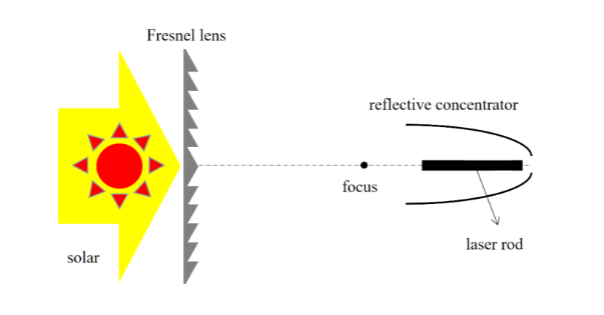
\includegraphics[width=0.65\textwidth]{images/setup.png}
		\end{figure}

    \begin{block}{Problems to solve:}
      \begin{enumerate}
				\item<2-> Build a framework for physically accurate raytracing
        \item<3-> Calculate absorbed power
        \item<4-> Optimize mirror shape
      \end{enumerate}
    \end{block}
		
    \end{frame}
  }

  { % Outline
    \setbeamertemplate{footline}{}
    \begin{frame}[noframenumbering]{Outline}
      \tableofcontents
    \end{frame}
  }
  \section{Optics}
		\begin{frame}[fragile]{Reflection}
		A ray is reflected by creating a new ray with the origin at the intersection
		point and the direction determined by the incident angle.

		\bigskip

		\begin{equation*}
			\theta_1 = \theta_2
		\end{equation*}

		\bigskip

		where $\theta_1$ is the incident angle and $\theta_2$ is the reflection angle.
    \end{frame}

		\begin{frame}[fragile]{Refraction}
		Refraction is modelled accurately by Snells' law:

		\begin{equation*}
			n_1 \sin (\theta_1) = n_2 \sin (\theta_2)
		\end{equation*}

		where $n_1$, $n_2$ are the indices of refraction.

		\begin{figure}
		\centering
		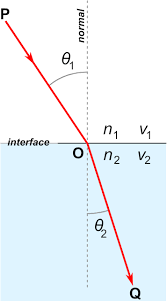
\includegraphics[width=0.25\textwidth]{images/snell.png}
		\end{figure}

    \end{frame}

		\begin{frame}[fragile]{Fresnel Laws}
		The transmitted and reflected power can be calculated with the transmission- and 
			reflection rates given by Fresnel's laws.\\
			These are dependent on the orientation of the polarization of the incident
			ray (perpendicular or parallel) to the surface:\\

		\begin{equation*}
			R_{\perp} = \frac{\sin^2(\theta_1 - \theta_2)}{\sin^2(\theta_1 + \theta_2)}
		\end{equation*}

		\begin{equation*}
			R_{\parallel} = \frac{\tan^2(\theta_1 - \theta_2)}{\tan^2(\theta_1 + \theta_2)}
		\end{equation*}

		\begin{equation*}
			T_{\perp} = 1 - R_{\perp}
		\end{equation*}

		\begin{equation*}
			T_{\parallel} = 1 - R_{\parallel}
		\end{equation*}
    \end{frame}

	\begin{frame}[fragile]{Fresnel Laws contd.}
		For now unpolarized light is assumed and only one refraction takes place so the total
		rates are:

		\begin{equation*}
			R_{total} = \frac{R_{\perp} + R_{\parallel}}{2}
		\end{equation*}

		\begin{equation*}
			T_{total} = \frac{T_{\perp} + T_{\parallel}}{2}
		\end{equation*}
    \end{frame}

	\begin{frame}[fragile]{Sellmeier Equation}
		Dependency of the refractive index on the wavelength of light is modelled
		using the Sellmeier equation.
		\begin{equation*}
        n^2(\lambda) = 1 + \sum_i \frac{B_i \lambda^2}{\lambda^2 - C_i}
    	\end{equation*}

		Here the $B_i$ and $C_i$ are empirically determined coefficients.
	\end{frame}


	\section{Ray Tracing}
    \begin{frame}[fragile]{Parametrization}
		
		All points along a ray are described as follows:

		\begin{equation*}
			\boldsymbol{r}(t) = \boldsymbol{o} + t \cdot \boldsymbol{d}
		\end{equation*}

		Testing intersections against primitives involves solving for the parameter $t$.\\
		\textbf{Example:} Axis aligned box intersection\\
		
		\begin{figure}
		\centering
		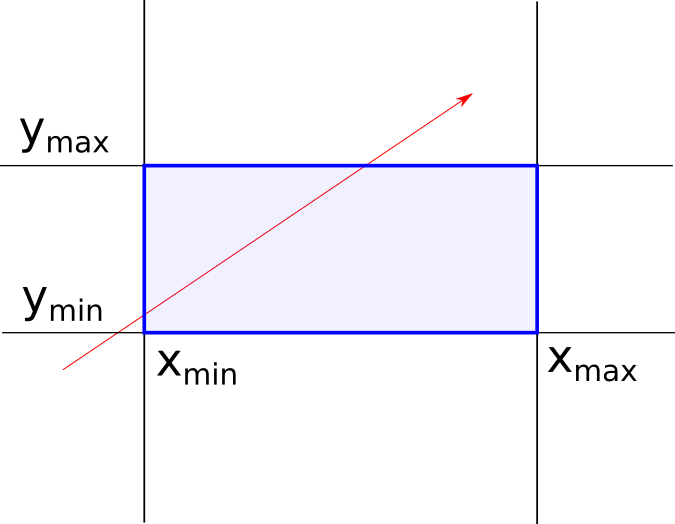
\includegraphics[width=0.5\textwidth]{images/aabb.png}
		\end{figure}
    \end{frame}

    \begin{frame}[fragile]{Parametrization contd.}
			\textbf{Solution:} \\
			\bigskip
			
		\begin{lstlisting}[language=C++]
  	float tx1 = (xmin - ray.origin.x) / ray.direction.x;
  	float tx2 = (xmax - ray.origin.x) / ray.direction.x;

  	float tmin = min(tx1, tx2);
  	float tmax = max(tx1, tx2);

  	float ty1 = (ymin - ray.origin.y) / ray.direction.y;
  	float ty2 = (ymax - ray.origin.y) / ray.direction.y;

  	tmin = max(tmin, glm::min(ty1, ty2));
  	tmax = min(tmax, glm::max(ty1, ty2));
		\end{lstlisting}
		\bigskip
		Other primitives in 2D can be lines, cricles, etc.\\
		Or in 3D triangles, quads, spheres, etc.\\
		\bigskip
		All objects in a scene need to be built with a collection of such primitives.
    \end{frame}

    \begin{frame}[fragile]{Scene Tracing}
			If a ray hits an object new rays are genertated according to its type
			of surface (reflection, refraction).\\
			\bigskip
			These new rays are traced again through the scene.\\
			\bigskip
			$\implies$ Recurse until a desired "depth".\\
			\bigskip
			An object is intersected if one of its primitives is hit.\\
			\bigskip
			$\implies$ Need to check each primitive of every object in the scene.\\
			\bigskip
			Runtime of a scene tracing step with $N$ objects with $M$ primitives each:

			\begin{equation*}
				O(N * M)
			\end{equation*}
    \end{frame}

    \begin{frame}[fragile]{Hierarchical Bounding Volumes}
			Performance optimization:\\
			\bigskip
      \begin{enumerate}
				\item<2-> Preprocessing: Attach a bounding box around each object and 
					recursively subdivide.
				\item<3-> Tracing: Check if ray hits bounding box. If yes recursively check its
					subdivisions.
      \end{enumerate}
			\bigskip
			Runtime of a scene tracing step with $N$ objects with $M$ primitives each
			and 5 recursive subdivisions:

			\begin{equation*}
				O(N * (5*4 + M/4^5)) = O(N * M/1024)
			\end{equation*}
    \end{frame}

    
    \begin{frame}[fragile]{Generating Rays and Random Sampling}
		The goal is to randomly generate a cone of rays originating in the focus
		of the fresnel lens.\\
		\bigskip
		$\implies$ Uniformly sample the opening angle around a direction vector.

		\begin{figure}
		\centering
		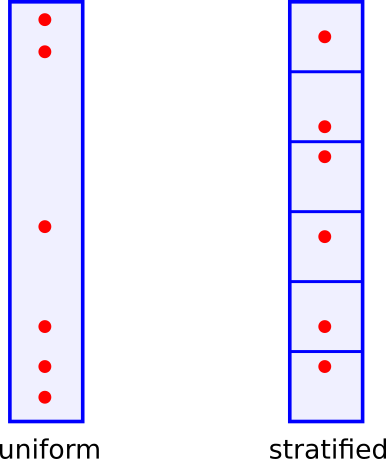
\includegraphics[width=0.3\textwidth]{images/stratified.png}
		\end{figure}

		\bigskip
		$\implies$ Not ideal in this case (big gaps between rays)\\
		$\implies$ Better: Stratified Uniform Sampling
		\end{frame}

		\begin{frame}[fragile]{Inversion Method}
		In reality sunlight consists of unpolarized light with a specific frequency spectrum.\\
		Thus the rays need to carry information about their power, frequency and polarity.\\
		\bigskip
		$\implies$ Need mechanism to generate random samples $x$ according to 
			a given distribution density function $p(x)$ (gauss, poisson, sun spectrum, etc.)\\
		\bigskip
			\textbf{Inversion Method:}\\
      \begin{enumerate}
				\item<2-> Integrate(sum up) the distribution $p(x)$ in uniform steps $x$ and save
					the value for each step resulting in $P(x)$.
				\item<3-> Uniformly sample $\xi \in [0,1]$ and figure out in which interval it lies.
        \item<4-> Interpolate linearly within the interval and return resulting $x$ value.
      \end{enumerate}

		\bigskip
		\bigskip
		Frequencies and polarisations of rays are not implemented as of yet.
    \end{frame}

		\begin{frame}[fragile]{Inversion Method contd.}
		\begin{figure}
		\centering
		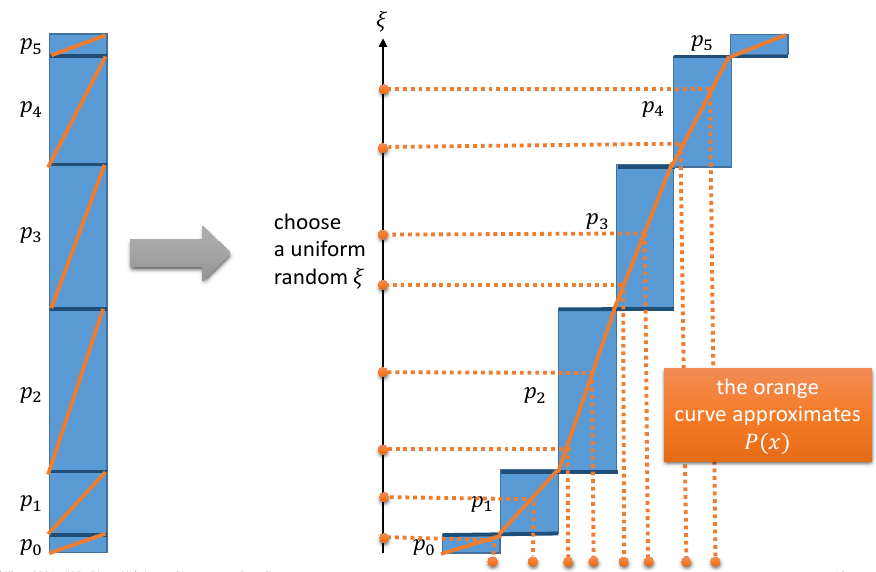
\includegraphics[width=0.8\textwidth]{images/inversion.png}
		\end{figure}
    \end{frame}


	
	\begin{frame}[fragile]{Mirror}
			Mirror consists of 2D line segments arranged by a 1D shape function (parabolic for testing
			purposes).

			\begin{figure}
			\centering
			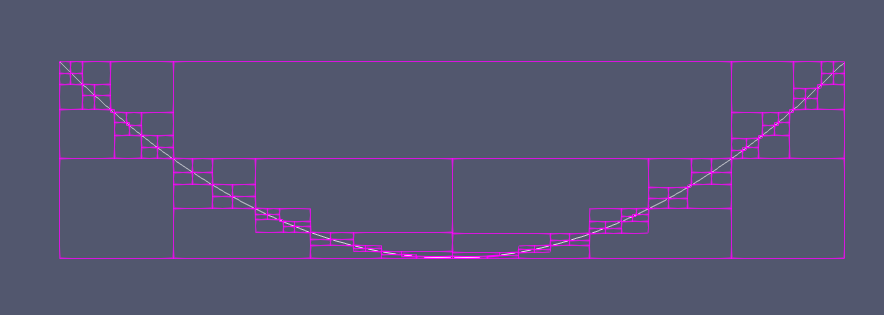
\includegraphics[width=0.8\textwidth]{images/mirror.png}
			\end{figure}
    \end{frame}

    \begin{frame}[fragile]{Crystal}
			The laser crystal is a 2D Box with an internal grid structure and grid tracing algorithm.\\
			Rays need to be traced through cells \textbf{in order}\footnote{A Fast Voxel Traversal Algorithm for Ray Tracing, John Amanatides, Andrew Woo, University of Toronto} because 
			of the absorbed energy calculation.\\

			\begin{figure}
			\centering
			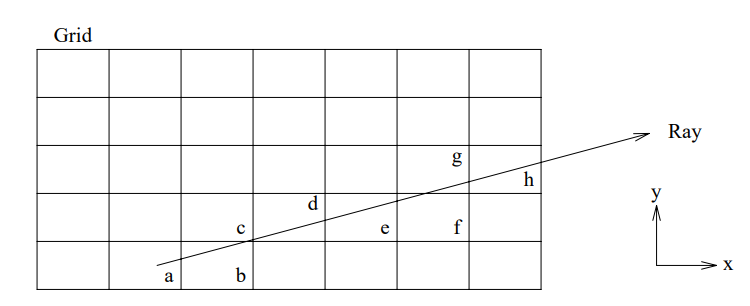
\includegraphics[width=0.8\textwidth]{images/grid.png}
			\end{figure}
    \end{frame}

		\begin{frame}[fragile]{Calculating Absorbed Power}
			The remaining power of a ray passing through the crystal is calculated by
			the Lambert law of absorption:

			\begin{equation*}
				I_{out} = I_{in} \cdot e^{-\alpha d}
			\end{equation*}

			where $\alpha$ is the absorption coefficient $d$ is the distance travelled
			through a cell.\\
			Thus the absorbed power is:

			\begin{equation*}
				I_{abs} = I_{in} - I_{out}
			\end{equation*}

			In reality the $\alpha$ is frequency dependent but this is not implemented yet.
    \end{frame}

	\begin{frame}[fragile]{Framework Overview}
	\begin{center}
	\resizebox{2.2in}{!}{
	\begin{tikzpicture}
    \begin{umlpackage}{Tracing}
    \umlsimpleclass[x=0, y=4]{IntersectResult2D}
    \umlsimpleclass[x=6, y=4]{AABB2D}
    \umlsimpleclass[type=interface, x=4, y=2]{Shape2D}
    \umlsimpleclass[x=9, y=3]{Line2D}
    \umlsimpleclass[x=9, y=2]{BoundingBox2D}
    \umlsimpleclass[x=9, y=1]{Sphere2D}

    \umlsimpleclass[type=interface, x=4, y=-2]{Object2D}
    \umlsimpleclass[x=9, y=-1]{Mirror2D}
    \umlsimpleclass[x=9, y=-2]{ThinLens2D}
    \umlsimpleclass[type=interface, x=9, y=-3]{Medium2D}
    \umlsimpleclass[x=9, y=-5]{Grid2D}
    
    \umlsimpleclass[x=0, y=-5]{Ray2D}


    \umlsimpleclass[x=0, y=-2]{Scene2D}
    
    \umlimpl[]{Line2D}{Shape2D}
    \umlimpl[]{BoundingBox2D}{Shape2D}
    \umlimpl[]{Sphere2D}{Shape2D}
    \umluniassoc[anchor1=70, geometry=|-]{Shape2D}{AABB2D}
    \umldep[anchor1=110, geometry=|-]{Shape2D}{IntersectResult2D}
    \umlimpl{Mirror2D}{Object2D}
    \umlimpl{ThinLens2D}{Object2D}
    \umlinherit{Medium2D}{Object2D}
    \umlimpl{Grid2D}{Medium2D}

    \umlunicompo{Object2D}{Shape2D}
    \umlunicompo{Scene2D}{Object2D}

    \umldep{Scene2D}{IntersectResult2D}
    \umldep{Scene2D}{Ray2D}

    \end{umlpackage}

    \begin{umlpackage}{Utilities}
        \umlsimpleclass[x=3, y=8]{VtkWriter}
        \umlsimpleclass[x=3, y=7]{CsvWriter}
        \umlsimpleclass[x=3, y=6]{CsvReader}
        \umlsimpleclass[x=6, y=8]{Timer}
        \umlsimpleclass[x=6, y=7]{ArgsParser}
        \umlsimpleclass[x=6, y=6]{FunctionUtils}
    \end{umlpackage}

    \begin{umlpackage}{NOMAD}
        \umlsimpleclass[x=9.5, y=8]{MADS}
        \umlsimpleclass[x=9.5, y=7]{BiMADS}
    \end{umlpackage}

    \begin{umlpackage}{Maths}
        \umlsimpleclass[type=interface, x=-0.5, y=8]{Sampler}
        \umlsimpleclass[x=-0.5, y=7]{Physics}
    \end{umlpackage}

    \umldep{Tracing}{Maths}
    \umldep{Tracing}{Utilities}
    \umldep{Tracing}{NOMAD}
    \end{tikzpicture}
	}
	\end{center}
	\end{frame}

	\section{Optimization}

	\begin{frame}[fragile]{Problem}
		\emph{Goal}: Optimize both total absorbed power and variance across the crystal\\
		\bigskip
		$\Rightarrow$ Should result in a better and more powerful beam (verification in ASLD)\\
		\bigskip
		$\Rightarrow$ Need an algorithm to handle two objective functions at the same time (biobjective optimization)\\
		\bigskip
		Additional problem: noisy and nonsmooth, computationally expensive objective functions!
	
	\begin{figure}
        \centering
        \begin{tabular}{c c}
        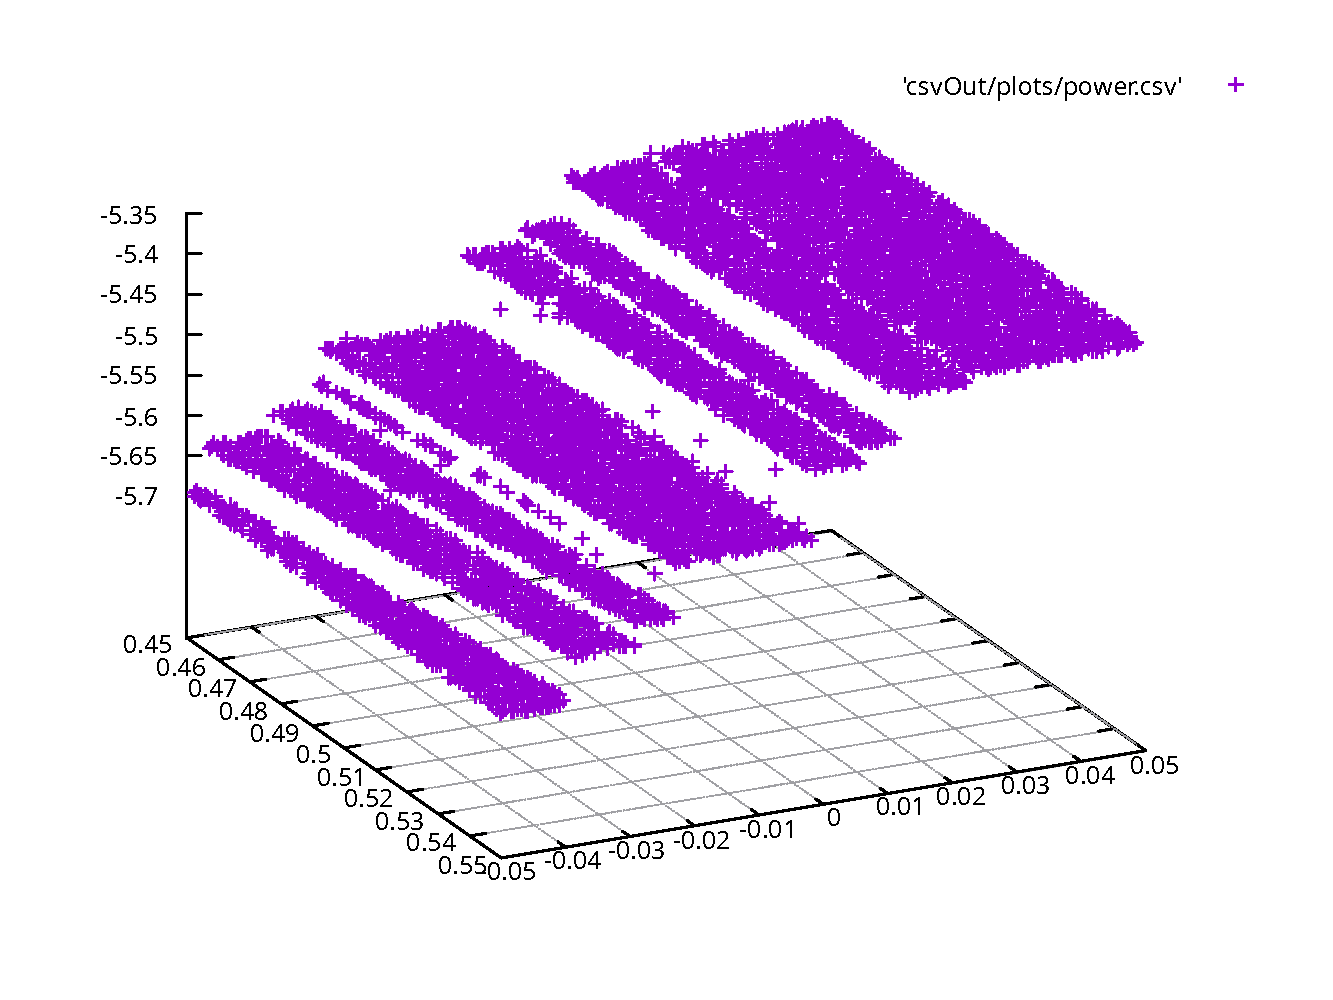
\includegraphics[width=0.4\textwidth]{images/discontinuity.pdf} &
        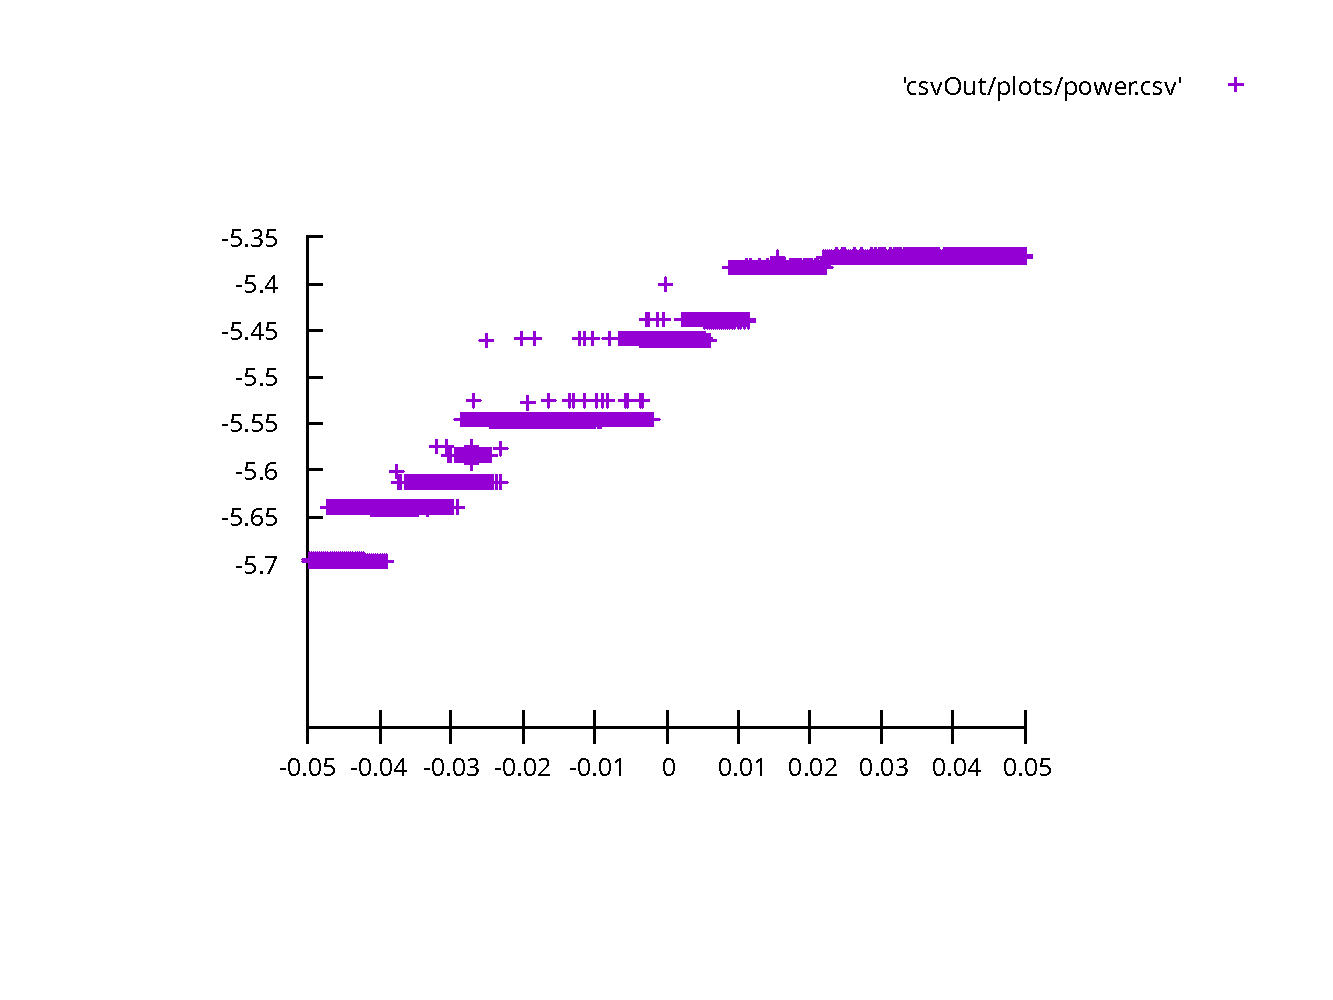
\includegraphics[width=0.4\textwidth]{images/noisyness.pdf}
        \end{tabular}
    \end{figure}

	\end{frame}

	\begin{frame}[fragile]{Derivative-Free Optimization}
		Minimization problem:

    	\begin{equation*}
        	\begin{gathered}
        	\text{Find} \quad \vec{x}_{min} \in \Omega \subseteq \mathbb{R}^n \quad \text{s.t.}\\
        	f(\vec{x}_{min}) \leq f(\vec{x}) \quad \forall \vec{x} \in \Omega
        	\end{gathered} 
    	\end{equation*}

		Global optimization is not possible anyway for non-convex functions.\\
		Problem: Gradient is not available, or easily computable!\\
		Use Derivative-Free algorithms, not relying on derivatives of objective functions\\
		\bigskip
		$\Rightarrow$ Should be used as last resort, only if little or no information can be exploited\\
		\bigskip
		$\Rightarrow$ Objectives are treated as black-box functions, where the goal is to also use as little
		actual evaluations as possible (caching, etc.)\\
		\bigskip
		$\Rightarrow$ Optimality is often defined in an alternative way, to e.g. gradient search algorithms\\
		\bigskip
		Types of BBO: Simplex-Methods, Direct-Search-Methods, Model-Based-Methods etc.
	\end{frame}

	\begin{frame}[fragile]{MADS}
		Mesh Adaptive Direct Search is a Directional Direct Search method, using two different
		meshes in order to achieve a stronger optimality criterium than e.g. pattern search methods.\\
		\bigskip
		
		\begin{block}{Main Idea:}
      	\begin{enumerate}
			\item<2-> Generate two different meshes (only conceptually)
        	\item<3-> Let mesh sizes shrink at different rates
        	\item<4-> Evaluate black-box functions only at intersections of the two meshes
      	\end{enumerate}
		\bigskip
		$\Rightarrow$ Optimality defined by via the Clarke generalized gradient
    \end{block}
	\end{frame}

	\begin{frame}[fragile]{MADS}
		Mesh Adaptive Direct Search is a Directional Direct Search method, using two different
		meshes in order to achieve a stronger optimality criterium than e.g. pattern search methods.\\
		\bigskip
		
		\begin{block}{Main Idea:}
      	\begin{enumerate}
			\item<2-> Generate two different meshes (only conceptually)
        	\item<3-> Let mesh sizes shrink at different rates
        	\item<4-> Evaluate black-box functions only at intersections of the two meshes
      	\end{enumerate}
		\bigskip
		$\Rightarrow$ Optimality defined by via the Clarke generalized gradient\\
		\bigskip
		$\Rightarrow$ Can be extended and used in a biobjective optimization problem!\\
    \end{block}
	\end{frame}

	\begin{frame}[fragile]{Clarke's Calculus}
		\begin{definition}
        \label{def:generalized_deriv}
        Let $X$ be Banach, $\vec{v} \in X$ some direction and 
        $f : X \rightarrow \mathbb{R}$ a real valued
        function that is locally Lipschitz continuous.
        The generalized directional derivative or Clarke directional
        derivative of $f$ at $\vec{x}$ in direction $\vec{v}$ is given by

        \begin{equation}
            f^{\circ}(\vec{x};\vec{v}) = 
            \lim_{y \rightarrow x; \lambda \downarrow 0} \sup
             \frac{f(\vec{y} + \lambda \vec{v}) - f(\vec{y})}{\lambda}
        \end{equation}
    	\end{definition}

		\begin{definition}
        The Clarke generalized gradient of $f$ at $\vec{x}$ is
        \begin{equation}
            \partial f(\vec{x}) = 
            \{\xi \in X : f^{\circ}(\vec{x}; \vec{v}) >
             \langle \vec{\xi}, \vec{v} \rangle\}
             \quad \forall \vec{v} \in X
        \end{equation}
	    \end{definition}


		\end{frame}

	\begin{frame}[fragile]{Clarke's Calculus}
		\begin{definition}
        \label{def:stationary_clarke}
        A point $\vec{\hat{x}}$ is called a Clarke stationary point,
        if the following holds
        
        \begin{equation}
            f^{\circ}(\vec{\hat{x}}; \vec{v}) \geq 0 \quad \forall
             \vec{v} \in \mathbb{R}^n
            \Longleftrightarrow
            0 \in \partial f(\vec{\hat{x}})
        \end{equation}
    	\end{definition}

		$\Rightarrow$ MADS produces Clarke stationary points!\\
		\bigskip
		$\Rightarrow$ Pattern serach does not in general!\\
		\bigskip
		$\Rightarrow$ Search directions need to be asymptotically dense!\\
	\end{frame}
	
	\begin{frame}[fragile]{GPS Frames}
	\begin{figure}
    \centering
	\resizebox{4.0in}{!}{
    \import{images/}{gps.pdf_tex}
	}
    \end{figure}
	\end{frame}

	\begin{frame}[fragile]{MADS Frames}
    \begin{figure}
    \centering
	\resizebox{4.0in}{!}{
    \import{images/}{mads.pdf_tex}
	}
    \end{figure}

	\end{frame}

	\begin{frame}[fragile]{Pareto Optimality}
	\begin{definition}
        \label{def:pareto_dominance}
        Let $\vec{u},\vec{v} \in X$ be two points of the multiobjective
        function $F: X \rightarrow Y$.
        \begin{itemize}
            \item $\vec{u} \preceq \vec{v}$ ($\vec{u}$ weakly dominates $\vec{v}$)
            $\Longleftrightarrow f_i(\vec{u}) \leq f_i(\vec{v}) \; \forall i \in \{1,\dots,p\}$   

            \item $\vec{u} \prec \vec{v}$ ($\vec{u}$ dominates $\vec{v}$)
            $\Longleftrightarrow \vec{u} \preceq \vec{v} \; \text{and} \; 
            f_j(\vec{u}) < f_j(\vec{v}) \; \text{for at least one} \; j \in \{1,\dots,p\}$   

            \item $\vec{u} \sim \vec{v}$ ($\vec{u}$ is indifferent to $\vec{v}$)
            $\Longleftrightarrow \; \text{$\vec{u}$ does not dominate $\vec{v}$ and $\vec{v}$
            does not dominate $\vec{u}$}$  
        \end{itemize}
    \end{definition}
	\end{frame}

	\begin{frame}[fragile]{Pareto Optimality}
	\begin{figure}
        \centering
        \resizebox{0.7\textwidth}{!}{\import{images/}{dominance_zones.pdf_tex}}
    \end{figure}
	\end{frame}

	\begin{frame}[fragile]{Pareto Optimality}
	\begin{definition}
        \label{def:optimality_multi}
        Let $\vec{x} \in X$ be a point of the multiobjective function $F: X \rightarrow Y$.
        \begin{itemize}
            \item $\vec{x}$ is globally Pareto optimal (just called Pareto optimal) 
            $\Longleftrightarrow$
            There exists no $\vec{y}$ s.t. $\vec{y} \prec \vec{x}$.
            If $\vec{x}$ is Pareto optimal then $F(\vec{x})$ is called
            Pareto efficient.

            \item $\vec{x}$ is locally Pareto optimal $\Longleftrightarrow$
            There exists an $\epsilon, \sigma > 0$ for which the set
            $\{\vec{y} \in B_{\epsilon}(\vec{x}) \cap X \, | \, \vec{y} \prec \vec{x},\, 
            F(\vec{y}) \in B_{\sigma}(F(\vec{x})) \}$ is empty.
            If $\vec{x}$ is locally Pareto optimal then $F(\vec{x})$ is called
            locally Pareto efficient.
        \end{itemize}
    \end{definition}
	\end{frame}

	\begin{frame}[fragile]{Pareto Optimality}
	\begin{figure}
        \centering
        \resizebox{0.7\textwidth}{!}{\import{images/}{pareto_front.pdf_tex}}
    \end{figure}
	\end{frame}

	\begin{frame}[fragile]{BiMADS}
		Produces an approximation of the Pareto front!\\
		\begin{block}{Main Idea:}
      	\begin{enumerate}
			\item<2-> Initially run MADS and save all Pareto optimal points
        	\item<3-> Generate a single objective formulation by a reference point approach
        	\item<4-> Run MADS and repeat step 2
        	\item<5-> Pareto optimal points along the way are returned as Pareto front
      	\end{enumerate}
		\end{block}
		\bigskip
		\bigskip
		$\Rightarrow$ Implementation used from the NOMAD library\\
	\end{frame}

	\section{Results}

	\begin{frame}[fragile]{Setup}
	\begin{figure}
        \centering
		\resizebox{\textwidth}{!}{
        \import{images/}{setup.pdf_tex}
		}
    \end{figure}
	\end{frame}

	\begin{frame}[fragile]{Results}
		\resizebox{\textwidth}{!}{
		\begin{tabular}{| p{2cm} | c | c | c | c | c | c | c |}
			\hline
			Setup & Pump power & Absorbed Power[W] & Variance[W] & cw-Output[W] & opt.-to-opt. Eff. [\%] & Beam quality x & Beam quality y \\
			\hline
			Reference (algebraic) & 720 & - & - & 30.52 & 4.24 & 4.82 & 4.30 \\
			\hline
			Fixed mirror and crystal distance & 720 & 155.46 & 13.49 & 35.14 & 4.88 & 4.25 & 3.22 \\
			\hline
			Open mirror and crytsal distance (initial random search) & 690 & 186.76 & 2.50 & 38.22 & 5.54 & 4.03 & 1.96 \\
			\hline
			Open mirror and crytsal distance (pipe configuration) & 665 & 191.13 & 4.08 & 38.05 & 5.72 & 3.90 & 1.66 \\
			\hline
		\end{tabular}
		}
    \end{frame}

	\begin{frame}[fragile]{Fixed setup}
	\begin{figure}
        \centering
		\resizebox{\textwidth}{!}{
        \begin{tabular}{c c}
        \includegraphics[width=0.5\textwidth]{images/fixed_rand/start.png}
        \includegraphics[width=0.5\textwidth]{images/fixed_rand/0.png}
        \end{tabular}
		}
    \end{figure}
    \end{frame}

	\begin{frame}[fragile]{Fixed Setup}
    \begin{figure}
        \centering
		\resizebox{0.5\textwidth}{!}{
        \begin{tabular}{c c}
            \includegraphics[width=0.5\textwidth]{images/fixed_rand/1.png} &
            \includegraphics[width=0.5\textwidth]{images/fixed_rand/2.png} \\
            \includegraphics[width=0.5\textwidth]{images/fixed_rand/3.png} &
            \includegraphics[width=0.5\textwidth]{images/fixed_rand/4.png} \\
        \end{tabular}
		}
    \end{figure}
    \end{frame}

	\begin{frame}[fragile]{Open setup}
	\begin{figure}
        \centering
		\resizebox{\textwidth}{!}{
        \begin{tabular}{c c}
        \includegraphics[width=0.5\textwidth]{images/open_rand/start.png}
        \includegraphics[width=0.5\textwidth]{images/open_rand/0.png}
        \end{tabular}
		}
    \end{figure}
    \end{frame}

	\begin{frame}[fragile]{Open setup}
    \begin{figure}
        \centering
		\resizebox{0.5\textwidth}{!}{
        \begin{tabular}{c c}
            \includegraphics[width=0.5\textwidth]{images/open_rand/1.png} &
            \includegraphics[width=0.5\textwidth]{images/open_rand/2.png} \\
            \includegraphics[width=0.5\textwidth]{images/open_rand/3.png} &
            \includegraphics[width=0.5\textwidth]{images/open_rand/4.png} \\
        \end{tabular}
		}
    \end{figure}
    \end{frame}

	
	\begin{frame}[fragile]{Open setup - pipe configuration}
	\begin{figure}
        \centering
		\resizebox{\textwidth}{!}{
        \begin{tabular}{c c}
        \includegraphics[width=0.5\textwidth]{images/open_pipe/start.png}
        \includegraphics[width=0.5\textwidth]{images/open_pipe/0.png}
        \end{tabular}
		}
    \end{figure}
    \end{frame}

	\begin{frame}[fragile]{Open setup - pipe configuration}
    \begin{figure}
        \centering
		\resizebox{0.5\textwidth}{!}{
        \begin{tabular}{c c}
            \includegraphics[width=0.5\textwidth]{images/open_pipe/1.png} &
            \includegraphics[width=0.5\textwidth]{images/open_pipe/2.png} \\
            \includegraphics[width=0.5\textwidth]{images/open_pipe/3.png} &
            \includegraphics[width=0.5\textwidth]{images/open_pipe/4.png} \\
        \end{tabular}
		}
    \end{figure}
    \end{frame}




  { % Questions?
    \setbeamertemplate{footline}{}
    \begin{frame}[c,noframenumbering]
      \begin{center}
        Thanks for listening.\\
        {\bf Any questions/suggestions?}
      \end{center}
    \end{frame}
  }
	\end{document}

